\chapter{Introduction}\label{ch:Introduction}

The population of the earth is projected to increase substantially over the next half-century, potentially reaching as high as 10 billion globally by 2050 \cite{World2010}.  At the same time, any attempt to increase the quality of life of the existing population will necessarily involve increased energy consumption per capita, with a greater fraction of the earth approaching ``first-world'' consumption levels \cite{HDI2011}.  As such, worldwide energy consumption will likely continue to increase in the next few decades \cite{EIA2011,BP2010}

This increase in energy demand occurs in parallel with increased pressure on traditional energy sources.  Fossil fuels (oil, coal, and natural gas), while reliable sources of base-load power, nevertheless face issues.  Oil faces increasing cost and technical difficulty in capturing dwindling available reserves, as well as the potential for serious ecological damage from accidents (\eg the Deepwater Horizon offshore rig accident in 2010).  Coal, while more readily available (an estimated 257 billion tons of recoverable reserves in the US, lasting roughly 240 years at current consumption \cite{BP2010,EIA2013}), releases particulate matter into the atmosphere, with serious consequences both to the environment and to human health, as well as the greenhouse gases tied to deleterious climate change.  

Renewable energy sources have a certain ``green'' appeal, but each is subject to strict limitations on their implementation.  Solar and wind power suffer from a large degree of variability in their output, necessitating a combination of expensive energy storage methods or (often fossil-fuel based) backup production to handle shortfalls.  Hydroelectric and geothermal power are suitable for base-load power production, but are strictly restricted in their implementation by geographic concerns -- bluntly, there are relatively few locations where hydro or geothermal power generation is possible, and many of these have already been developed \gnote{cite for this?}.

Conventional -- that is, fission-based -- nuclear power can also supply carbon-free base-load power, with fuel reserves lasting through the next century.  While nuclear power does  suffer from the potential for extremely serious accidents (Fukushima, Chernobyl) it is, in general, highly safe.  However, public perception of nuclear power hinges on these safety concerns, limiting the expansion of nuclear power to meet increasing demand and the safe long-term handling of existing nuclear waste, as well as, ironically, preventing the replacement of an aging reactor fleet with newer, safer designs.

\emph{Fusion}, the nuclear process driving stellar cores, is a potentially highly attractive option for satisfying the world's growing energy needs in an efficient, environmentally-sound manner.  A fusion reactor would supply base-load power using only a small amount of an effectively inexhaustible fuel (readily available for harvesting from seawater), with no greenhouse gas emissions or meaningfully radioactive waste, and the physical impossibility of a major ``meltdown'' accident.  However, fusion remains in the experimental stage, with significant technical hurdles remaining before the development of a prototype fusion power plant.  This thesis will attempt to contribute to the understanding of one of these hurdles, regarding the requirement for efficient plasma behavior in a reactor scenario \note{reword this!}  Further reading on the development of fusion energy is available to the interested reader in several excellent references. \cite{Freidberg2007,Wesson2011,Chen1984} \nicesectionending
\gnote{reword last sentence...}

%%%%%%%%%%%%%%%%%%%%%%%%%%%%%%%%%%%%%%%%%%%%%%%%%%%%

\section{Plasmas for Fusion}\label{sec:intro_plasmas}

A \emph{plasma} is a gas to which sufficient energy has been applied to strip some or all of the electrons off the nuclei of its constituent atoms.  These ions and electrons freely interact with one another, behaving as coupled fluids.  Plasmas of interest for fusion research are comprised of light elements (typically Hydrogen or Helium), and are at extremely high temperatures, in excess of 100 million Kelvin ($10-20 \;\si{keV}$).  As these conditions are far in excess of the ionization energy for these elements, the plasma is dominated by collisions between its charged particles, rather than interactions with bound electron states.

\subsection{Plasma Parameters}\label{subsec:intro_params}

As the plasma is comprised of free charged particles, it responds strongly to electric and magnetic fields.  In the presence of a DC electric field (externally applied, or generated by an imbalance of positive and negative charge in the plasma), the plasma will rearrange itself to screen out the field.  This effect breaks down at short length scales, at which there is an insufficient number of charge carriers to rearrange and counter the field -- the characteristic scale for this effect is the Debye Length, given by

\begin{equation}\label{eq:debye}
 \lambda_D = \sqrt{ \frac{\varepsilon_0 T}{n e^2} }
\end{equation}

\noindent At size scales significantly larger than $\lambda_D$, this will enforce an approximately balanced electric charge in the plasma, termed ``quasi-neutrality''.  This is reflected in the number densities of electrons and multiple ion species $j$, each with charge $Z_j$, by the relation

\begin{equation}\label{eq:quasineutral}
 n_e = \sum_j{n_j Z_j}
\end{equation}

\noindent In a multiple-ion species plasma, we may also define an effective ion charge

\begin{equation}\label{eq:Zeff}
 Z_{eff} = \frac{1}{n_e} \sum_j{n_j Z_j^2}
\end{equation}

The electrostatic force driving this charge redistribution induces a ``ringing'' oscillation in the plasma, at the characteristic plasma frequency $\omega_p$:

\begin{equation}\label{eq:omegap}
 \omega_p = \sqrt{ \frac{ne^2}{\varepsilon_0 m_e} }
\end{equation}

\noindent This natural oscillation in the plasma also has the effect of screening AC electric fields varying at frequencies $\omega < \omega_p$.

Coulomb collisions between charged particles in the plasma tend to drive magnetically-confined plasmas into thermal equilibrium, with the velocity distribution for a species given by the Maxwellian

\begin{equation}\label{eq:maxwell}
 f(v) = n \left( \frac{m}{2\pi T} \right)^{3/2} \mbox{exp}\left(-\frac{mv^2}{2T} \right)
\end{equation}

\noindent These collisions also cause the plasma to emit a continuous spectrum of Bremsstrahlung radiation.  For a plasma in thermal equilibrium, integration over the full spectrum gives for the total radiated power

\begin{equation}\label{eq:brems}
 P_{Brems} = \left( \num{5.35e-37} \right) n_e^2 Z_{eff} \sqrt{T}
\end{equation}

\noindent representing a consistent source of heat loss from the plasma.

\subsection{Fusion Fuels}\label{subsec:intro_fuels}

Fusion collectively refers to the class of nuclear reactions merging lighter nuclei into a single heavier element.  While fusion reactions for elements lighter than iron are generally exothermic, as they form nuclei with greater binding energy per nucleon (see \cref{fig:bindingenergy}), the most common and readily attainable involve isotopes of hydrogen or helium, the most promising candidates for which are shown below.

\begin{align}
 {}^2\si{D} + {}^2\si{D} &\rightarrow {}^3\si{T} + \si{p} + \SI{4.03}{\mega\electronvolt}\label{eq:dd1}\\
 {}^2\si{D} + {}^2\si{D} &\rightarrow {}^{3}\si{He} + \si{n} + \SI{3.27}{\mega\electronvolt}\label{eq:dd2}\\
 {}^2\si{D} + {}^3\si{He} &\rightarrow {}^4\si{He} + \si{p} + \SI{18.3}{\mega\electronvolt}\label{eq:dhe3}\\
  {}^2\si{D} + {}^3\si{T} &\rightarrow {}^4\si{He} + \si{n} + \SI{17.6}{\mega\electronvolt}\label{eq:dt}
\end{align}

\noindent Here $\si{D}$ and $\si{T}$ indicate nuclei of deuterium and tritium, two heavy isotopes of hydrogen (one proton plus one and two neutrons, respectively).  The fusion reaction rate $R_f$ is given by

\begin{equation}\label{eq:rate}
 R_f = n_1 n_2 \langle \sigma v \rangle_{1,2}
\end{equation}

\noindent where $n_1$ and $n_2$ indicate the densities of the two fuel ions (\eg for deuterium-tritium fuel $n_1 n_2 = n_D n_T$, while for pure-deuterium fuel $n_1 n_2 = \frac{1}{2} n_D^2$ to remove double-counting of fuel ions) and $\langle \sigma v \rangle_{1,2}$ is a rate parameter incorporating the energy-dependent reaction cross-section averaged over the Maxwellian fuel distribution (\cref{eq:maxwell}).  In practice, the energy-dependent cross-section is empirically determined -- measured rate parameters $\langle \sigma v \rangle$ for the fuels of interest are shown in \cref{fig:xsection}.

\begin{figure}
 \pushtooutside
 \ffigbox[\FBwidth]{\caption{Binding energy per nucleon versus atomic mass number, with notable isotopes marked.  Reactions forming nuclei with higher binding energy are exothermic -- thus, fusion of elements lighter than ${}^{56}\si{Fe}$ or fission of elements heavier than ${}^{56}\si{Fe}$ releases energy. \cite{Krane}}\label{fig:bindingenergy}}{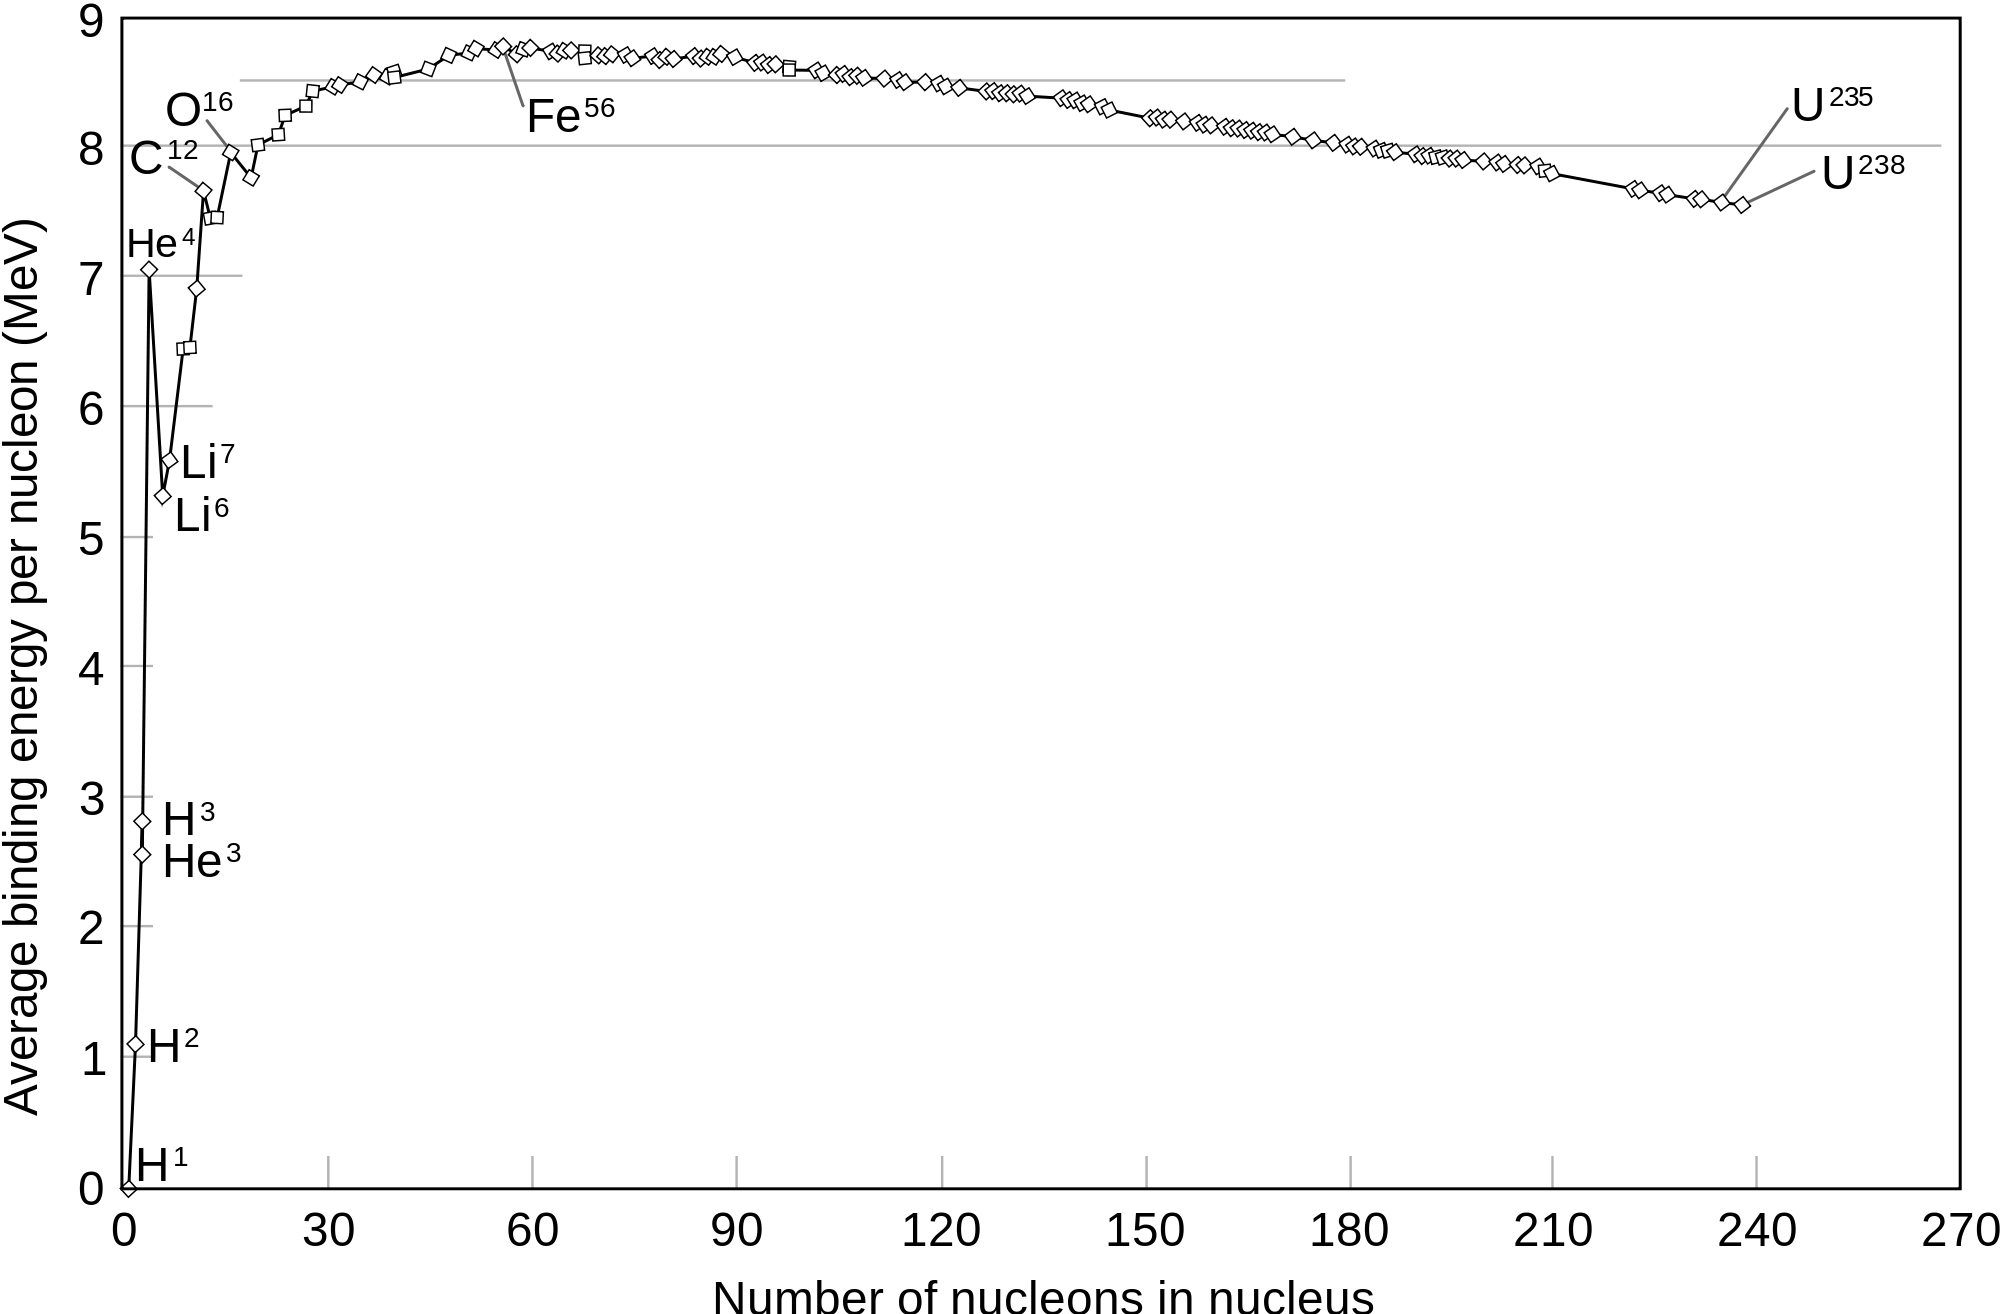
\includegraphics[width=150mm]{graphics/Introduction/bindingenergy.png}}
\end{figure}

\begin{figure}
 \pushtooutside
 \ffigbox[\FBwidth]{\caption{Reaction rate normalized to fuel density, expressed as the rate coefficient $\langle \sigma v \rangle$, for fusion fuels as a function of temperature.  Notably, deuterium-tritium fusion exhibits a higher peak reaction rate, as well as reaching that peak at a lower temperature, than other fuels.}\label{fig:xsection}}{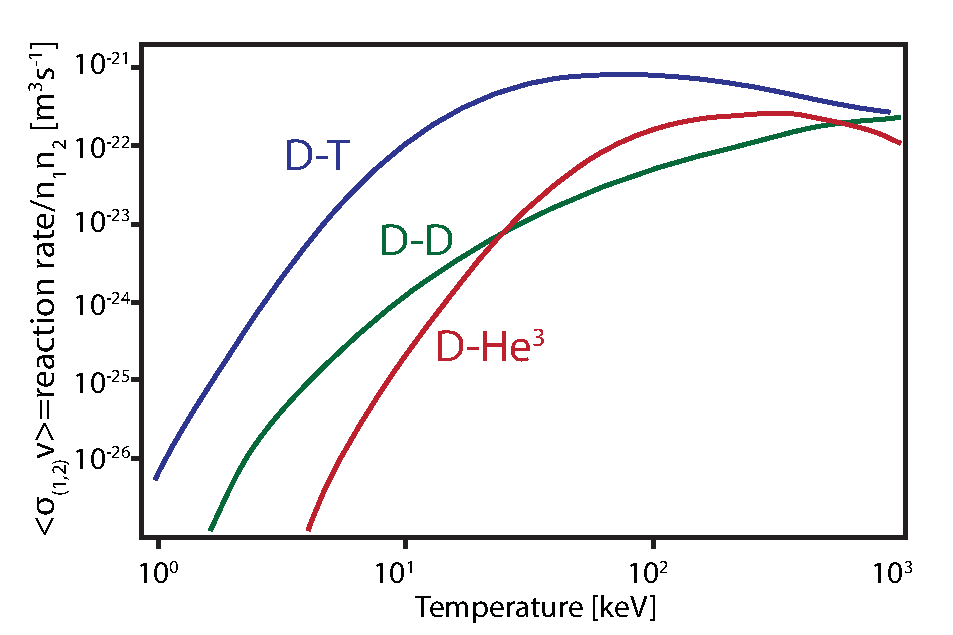
\includegraphics[width=150mm]{graphics/Introduction/reaction_xsections.pdf}}
\end{figure}

\gnote{pull cite for deuterium prevalence?}
Pure deuterium fuel (reactions shown in \cref{eq:dd1,eq:dd2}) is attractive from a research standpoint, due to the abundance and ease of use of deuterium.  Deuterium is a stable nucleus, obviating the need for radiation safety in the fuel system, and is naturally occurring in relative abundance (approximately $1/6420$ of hydrogen nuclei on earth are deuterium \note{cite}), allowing harvesting of deuterium fuel from seawater.  However, pure-deuterium reactions suffer from low energy output per reaction and a significantly lower reaction rate at feasible plasma conditions compared to other fuel options (see \cref{fig:xsection}), setting high performance requirements for a putative DD-burning reactor.

\gnote{citation for He-3 in lunar regolith?}
The $\si{D}-\si{He}^3$ reaction (\cref{eq:dhe3}) exhibits several desirable properties, namely an impressive energy yield per reaction, and the fact that the reaction produces only charged particles rather than the high-energy neutrons found in $\si{D}-\si{D}$ and $\si{D}-\si{T}$ reactions, which can cause significant damage to reactor materials.  However, as with $\si{D}-\si{D}$ fuel, the $\si{D}-\si{He}^3$ reaction suffers from a lower reaction rate at attainable conditions, as well as the fact that Helium-3 does not occur in economically usable quantities on Earth.  While off-planet sources of Helium-3 exist (for example, a useful quantity is present in the lunar regolith \note{cite}), this fuel remains the subject of speculation.

The deuterium-tritium reaction (\cref{eq:dt}) is considered the most promising for a first-generation fusion reactor, due to its high energy output per reaction and favorable reaction cross-section -- the rate parameter $\langle \sigma v \rangle_{DT}$ reaches its peak at a lower temperature, and reaches a greater absolute level than other fusion fuels.  However, $\si{D}-\si{T}$ operation is limited both by fuel sources, and reaction products.  $\si{D}-\si{T}$ fusion produces a $14 \;\si{MeV}$ neutron, carrying roughly 80\% of the energy released by the fusion reaction, which can damage unshielded reactor materials.  Moreover, while deuterium is stable and readily available, tritium is radioactive with a short half-life (roughly 12.3 years), so it is not naturally occurring in meaningful quantities on earth.   A reactor will solve both of these problems with a \emph{neutron blanket}, a neutron-absorbing structure surrounding the plasma.  This provides the necessary shielding for sensitive reactor 
components.  The heat generated in the blanket from neutron absorption will also be drawn off in a steam cycle to drive turbines, generating electricity from the reactor.  Finally, seeding the blanket with lithium allows the following reactions with fusion neutrons:

\begin{align}
 {}^6\si{Li} + \si{n}_{slow} &\rightarrow {}^4\si{He} + \si{T} + \SI{4.8}{MeV}\label{eq:Li6}\\
 {}^7\si{Li} + \si{n}_{fast} &\rightarrow {}^4\si{He} + \si{T} + \si{n} - \SI{8.7}{MeV}\label{eq:Li7}
\end{align}

\noindent the Lithium-6 reaction (\cref{eq:Li6}) absorbs ``slow'' neutrons (that is, neutrons that have thermalized to the blanket temperature via collisions) to produce tritium, plus additional heat.  Lithium-7 (\cref{eq:Li7}) is more likely to capture fast neutrons to produce tritium in an endothermic reaction; however, the reaction also acts as a neutron multiplier, as a free neutron is maintained through the reaction.  Using blankets enriched with ${}^6\si{Li}$, coupled with neutron multipliers, a reactor will target an over-unity tritium breeding ratio, with $>1$ tritons produced per neutron entering the blanket (\ie per tritium consumed in a fusion reaction).\nicesectionending

%%%%%%%%%%%%%%%%%%%%%%%%%%%%%%%%%%%%%%%%%%%%%%%%%%%%

\section{Magnetic Confinement}\label{sec:intro_magnetic}

\subsection{Basic Principles}\label{subsec:intro_basic}

The temperatures in excess of 100 million Kelvin necessary for fusion in a plasma are incompatible with any contact between solid reactor materials and the hot core of the plasma.  Magnetic confinement relies on the strong response of the charged particles comprising the plasma to magnetic fields, rather than a material wall, to retain the thermal pressure ($\sim 10 \;\si{atm}$ for a reactor) from the plasma.  The response of a charged particle to electric and magnetic fields is governed by the Lorentz force,

\begin{equation}\label{eq:lorentz}
 \vec{F} = q\left(\vec{E} + \vec{v} \times \vec{B}\right)
\end{equation}

\begin{figure}
 \pushtooutside
 \fcapside[50mm]{\caption{Electron and ion gyro orbits in an applied magnetic field.  Note that, due to the charge dependence in the Lorentz Force (\cref{eq:lorentz}), electrons and ions orbit in opposite directions relative to the magnetic field.}\label{fig:intro_gyro}}{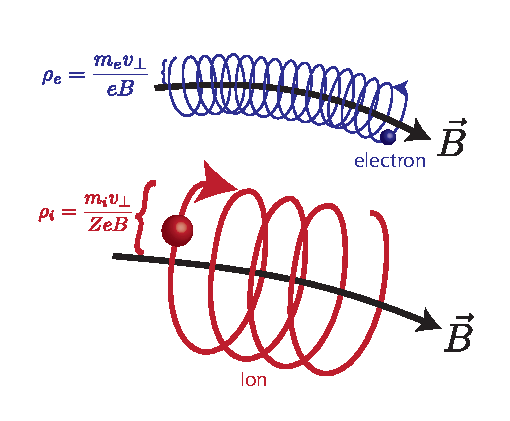
\includegraphics[width=85mm]{graphics/Introduction/gyro.pdf}}
\end{figure}

\noindent In a strong background magnetic field, the particle will move on a helical path along the magnetic field.  The $\vec{v} \times \vec{B}$ factor in the Lorentz Force causes the particle to experience no magnetic force parallel to the field, while velocity perpendicular to the field generates a force proportional to the velocity times the magnetic field, directed perpendicular to both -- thus the particle freely streams parallel to the field, but is trapped in a circular orbit perpendicular to it, termed ``gyro motion'', as depicted in \cref{fig:intro_gyro}.  The particle will orbit at the cyclotron frequency,

\begin{equation}\label{eq:omegac}
 \omega_c = \frac{qB}{m} \quad\Rightarrow\quad \omega_{ce} = \frac{eB}{m_e}, \quad \omega_{ci} = \frac{ZeB}{m_i}
\end{equation}

\noindent for electrons and ions of charge $Z$, respectively (note that for brevity we indicate the magnitude of vectors as scalar variables, \eg $B = \left|\vec{B}\right|$).  A particle with velocity perpendicular to the magnetic field $v_\perp$ (formally, $v_\perp = \left|\vec{v} \times \vec{B}\right|/B$) orbits at its gyroradius,

\begin{equation}\label{eq:gyroradius}
 \rho = \frac{v_\perp}{\omega_c} = \frac{mv_\perp}{qB}
\end{equation}

\noindent For a thermalized plasma, the perpendicular velocity will, on average, be the thermal velocity $v_t = \sqrt{2T/m}$, thus

\begin{equation}\label{eq:gyroradius2}
 \rho = \frac{\sqrt{2mT}}{qB}
\end{equation}

\noindent The introduction of a nonzero electric field drives additional motion for the particle in the form of a drift velocity -- the guiding center (that is, the average point about which the orbital motion of the particle gyrates) will shift with a bulk velocity (see \cite[\S 8.4]{Freidberg2007} for derivation)

\begin{equation}\label{eq:exb}
 \vec{v}_d = \frac{\vec{E} \times \vec{B}}{B^2}
\end{equation}

\noindent independent of particle charge, mass, or energy.

This restriction of particle motion perpendicular to field lines to short length scales (at fusion-relevant temperatures and magnetic fields, the gyroradius is typically $\sim 10^{-5} \;\si{m}$ for electrons and $\sim 10^{-3} \;\si{m}$ for ions) compared to the size of the plasma is central to the premise of magnetic confinement.  In the perpendicular direction, this scale restriction of particle motion permits a fluid treatment of the dynamics of the plasma.  Further simplification of the fluid model (see \cite[\S 2.3]{Freidberg1987} for detailed derivation) leads to the theory of \emph{magnetohydrodynamics} (MHD), the ``workhorse'' model describing plasma behavior.  A basic equilibrium in a confined plasma is described in MHD by the simple relation

\begin{equation}\label{eq:MHDeq}
 \nabla p = \vec{J} \times \vec{B}
\end{equation}

\noindent in which the outward force due to the plasma pressure gradient is balanced by an inward force from the interplay between magnetic fields and electric currents (expressed by the current density $\vec{J}$).  This interplay is readily illustrated in the simple one-dimensional case of an infinite straight cylinder of plasma -- in this case, the radially-outward $\nabla p$ force may be balanced by an axial current in the $\hat{z}$ direction with an azimuthal $\hat{\theta}$ magnetic field ($z$-pinch), an azimuthal current and axial field ($\theta$-pinch), or a superposition of the two (screw pinch).  However, all three of these options suffer from a lack of parallel confinement -- as the magnetic field does not restrict the free-streaming parallel motion of the plasma, these linear concepts (when reduced to a physical, non-infinite size!) suffer from plasma losses at the ends of the cylinder.  Despite efforts to restrict the parallel motion in a linear device (\eg the ``magnetic mirror,'' which pinches 
the 
magnetic field at the cylinder ends in order to reflect the parallel motion of particles with a force due to the field gradient \cite{Kesner1982}), end losses in linear devices proved incompatible with steady-state fusion conditions.  The clear solution, then, was to close the magnetic geometry such that the magnetic field lines have no ends: a \emph{torus.}

\subsection{Toroidal Configurations}\label{subsec:intro_toroidal}

\begin{figure}[h]
 \pushtooutside
 \fcapside[55mm]{\caption{Example geometry of a circular-cross-section tokamak plasma, describing a torus of major radius $R_0$ and minor radius $a$.  The poloidal coordinate is denoted $\theta$, and the toroidal coordinate is denoted $\Phi$.  Tokamak configurations are characterized by an applied toroidal field $B_T$ with a toroidal plasma current $I_p$, which in turn generates a poloidal magnetic field $B_p$.}\label{fig:intro_geometry}}{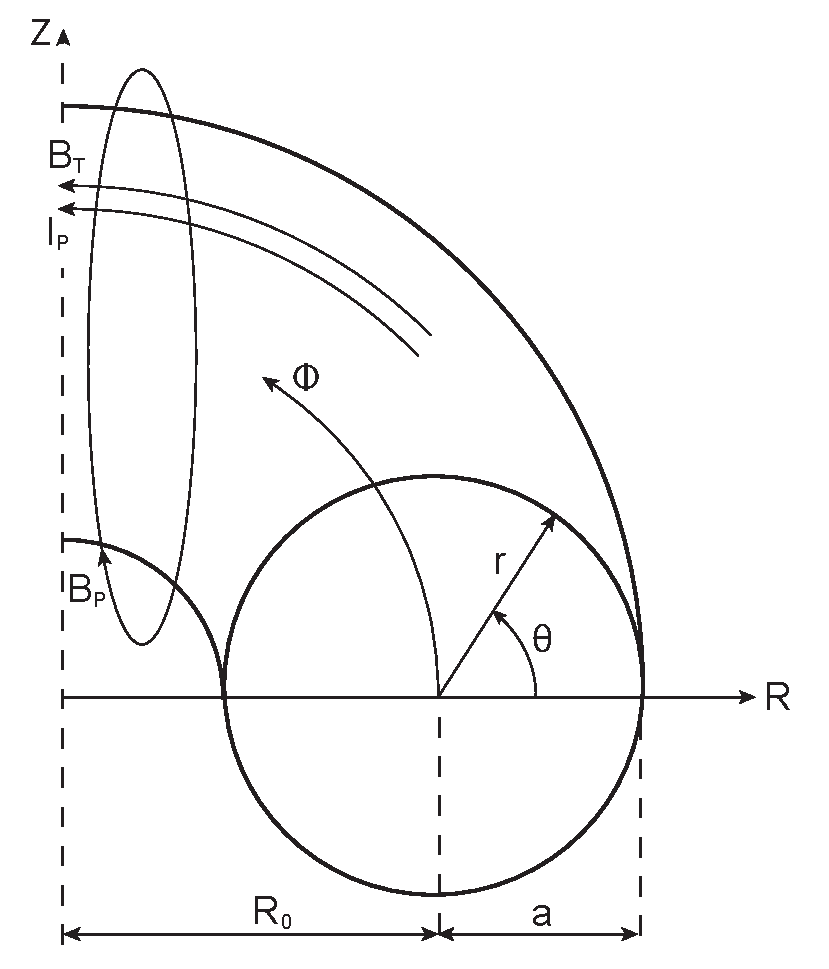
\includegraphics[width=90mm]{graphics/Introduction/geometry.pdf}}
\end{figure}

An example toroidal geometry is shown above in \cref{fig:intro_geometry}.  In comparison to the previous straight cylindrical geometry, the radial coordinate is replaced by a \emph{minor radius} $r$, measured from the center of the plasma column to its edge ($r=a$), while the \emph{major radius} $R_0$ denotes the radius of the torus itself measured from its center axis ($Z$ in \cref{fig:intro_geometry}) to the plasma axis.  The azimuthal cylindrical coordinate is replaced by the poloidal coordinate $\theta$, wrapping immediately about the plasma column.  The axial coordinate in the cylindrical system is replaced by the toroidal angle $\Phi$ wrapping around the center axis of the torus and describing a circuit along the plasma column.  As with the straight cylindrical case, the magnetic geometry may be described with toroidal and poloidal currents and magnetic fields balancing radially-outward thermal pressure.

However, introducing toroidal effects into the magnetic geometry gives rise to additional drift velocities, causing the guiding centers of particle gyro-orbits to shift (see \cite[\S 8.5-7]{Freidberg2007}).  Variation in the magnetic field strengths causes the $\nabla B$ drift, given by

\begin{equation}\label{eq:gradbdrift}
 \vec{v}_{\nabla B} = \frac{v_\perp^2}{2\omega_c} \frac{\vec{B} \times \nabla B}{B^2}
\end{equation}

\noindent while the toroidal twist in the magnetic field causes the curvature drift,

\begin{equation}\label{eq:curvaturedrift}
 \vec{v}_\kappa = \frac{v_\parallel^2}{\omega_c} \frac{\vec{R}_c \times \vec{B}}{R_c^2 B}
\end{equation}

\noindent where $v_\parallel$ is the particle velocity parallel to the magnetic field, $\omega_c$ is the species cyclotron frequency (\cref{eq:omegac}), and $\vec{R}_c$ is the radius of curvature of the field.  In the case of an applied toroidal magnetic field, these drifts are directed vertically in the $\hat{Z}$ direction, and are directed oppositely for electrons and ions due to the charge dependence in $\omega_c$.  The electric field resulting from this charge separation drives an outward $\vec{E} \times \vec{B}$ drift (see \cref{eq:exb}), breaking confinement.  This effect is countered by the addition of a poloidal field, which adds a helical twist to the guiding-center path to average out the separation due to particle drifts.  Concepts aiming for steady-state magnetic confinement of a plasma typically rely on generating this twist, termed the ``rotational transform,'' to maintain stable confinement.

\gnote{general cite for tokamaks, stellarators?}  
One of the most successful implementations of this concept for Magnetic Fusion Energy (MFE) is the \emph{tokamak} (a Russian acronym from \foreignlanguage{russian}{тороидальная камера с магнитными катушками}, \emph{toroidalnaya kamera s magnetnymi katushkami}, ``toroidal chamber with magnetic coils'').  The tokamak design is characterized by a strong toroidal magnetic field applied by external coils, with a poloidal field primarily generated by a current (termed the \emph{plasma current} $I_p$).  A schematic of the plasma and coil arrangement for a tokamak is shown in \cref{fig:intro_tokamak}.  By generating the rotational transform to the magnetic field using the plasma current, the tokamak design utilizes relatively simple planar magnetic coils, avoiding the significantly more complex three-dimensional coils used to generate the helical field in a \emph{stellarator} (the major competing design concept).\gnote{cite?}  However, the necessity for large ($>\SI{1}{\mega\ampere}$) plasma currents presents a 
significant engineering and physics challenge.  It is straightforward to generate the plasma current through a simple transformer action from a central solenoid in the torus (depicted in \cref{fig:intro_tokamak}) -- however, this AC-current-driven transformer action necessarily limits tokamaks to pulsed operation.  Generation of DC plasma current (via RF or neutral-beam-driven methods) is an active area of research in tokamak physics and engineering, but is outside the scope of this thesis.\gnote{point to refs in Wesson, maybe?}

\begin{figure}[t]
 \pushtooutside
 \ffigbox[\FBwidth]{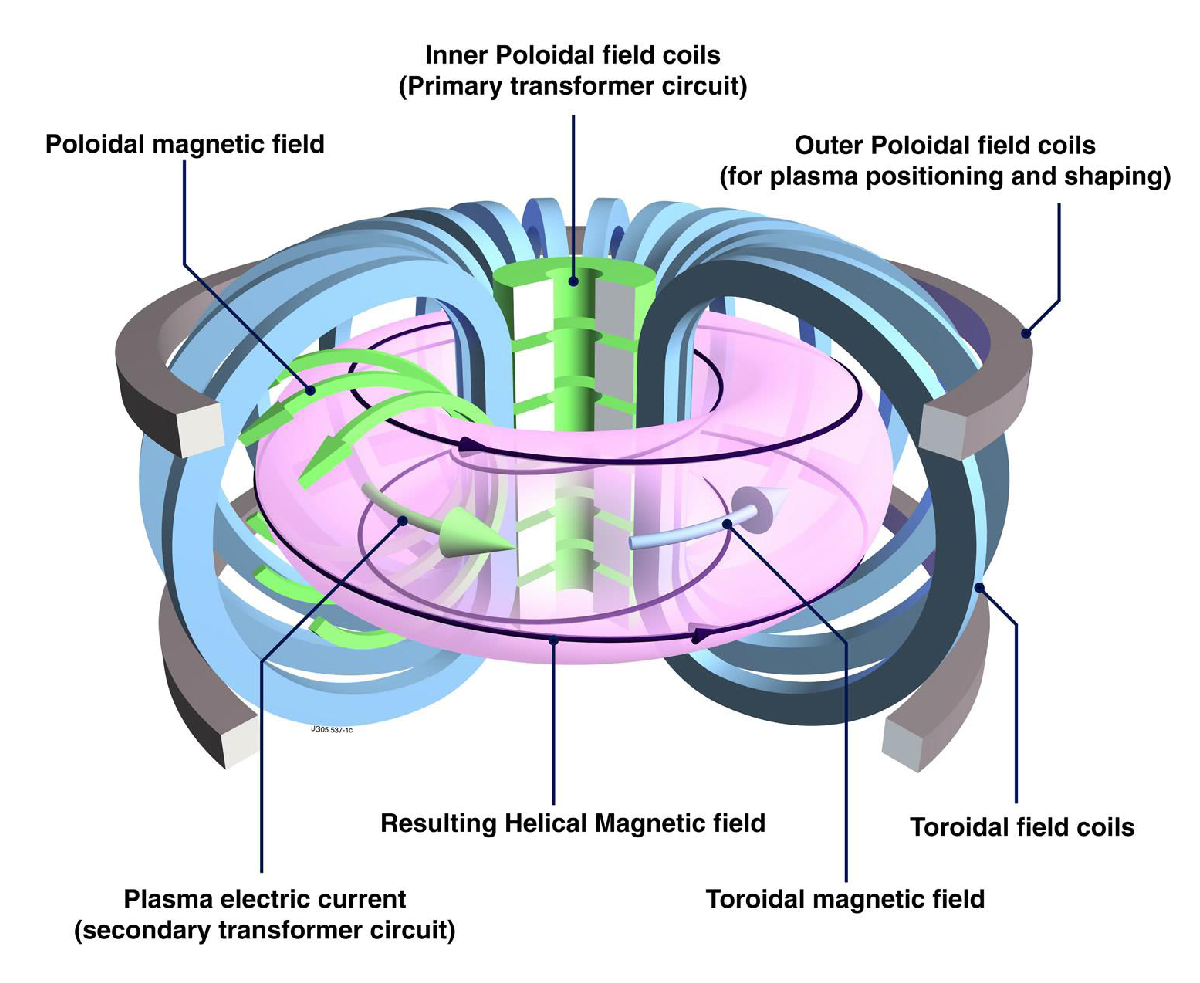
\includegraphics[width=150mm]{graphics/Introduction/tokamak.pdf}}{\caption{Schematic of a tokamak configuration, showing the plasma and magnetic coils.  The applied toroidal magnetic field is generated by the toroidal field coils (shown in blue).  A toroidal plasma current is generated by the center transformer, in turn generating a poloidal magnetic field (shown in green).  These combine to form the helical magnetic field.  The plasma shape and equilibrium is adjusted with the outer poloidal field coils (gray).}\label{fig:intro_tokamak}}
\end{figure}

Due to its regular, planar magnetic coils and continuous plasma current, tokamak equilibria are characterized by rotational symmetry about the center axis of the torus (\emph{axisymmetry}).  Solutions to the MHD equilibrium equation, \cref{eq:MHDeq}, thus reduce to a two-dimensional equation in $R$ and $Z$ (as $\partial/\partial \Phi \rightarrow 0$), given by the Grad-Shafranov Equation\gnote{Cite for GSE}:

\begin{equation}\label{eq:gradshafranov}
 \begin{aligned}
 \Delta^* \psi &= -\mu_0 R^2 \frac{dp}{d\psi} - \frac{1}{2} \frac{dF^2}{d\psi}\\
 \Delta^* \psi &= R^2 \nabla \cdot \left(\frac{1}{R^2} \nabla \psi \right) = R \frac{\partial}{\partial R} \left(\frac{1}{R} \frac{\partial \psi}{\partial R} \right) + \frac{\partial^2 \psi}{\partial Z^2}
 \end{aligned}
\end{equation}

\noindent where $F = RB_\phi$ encodes the toroidal field, $p$ is the thermal pressure, and $\psi$ describes the poloidal magnetic flux. \note{continue, describe magnetic flux, flux functions, plasma shaping}

\begin{figure}
 \pushtooutside
 \ffigbox[\FBwidth]{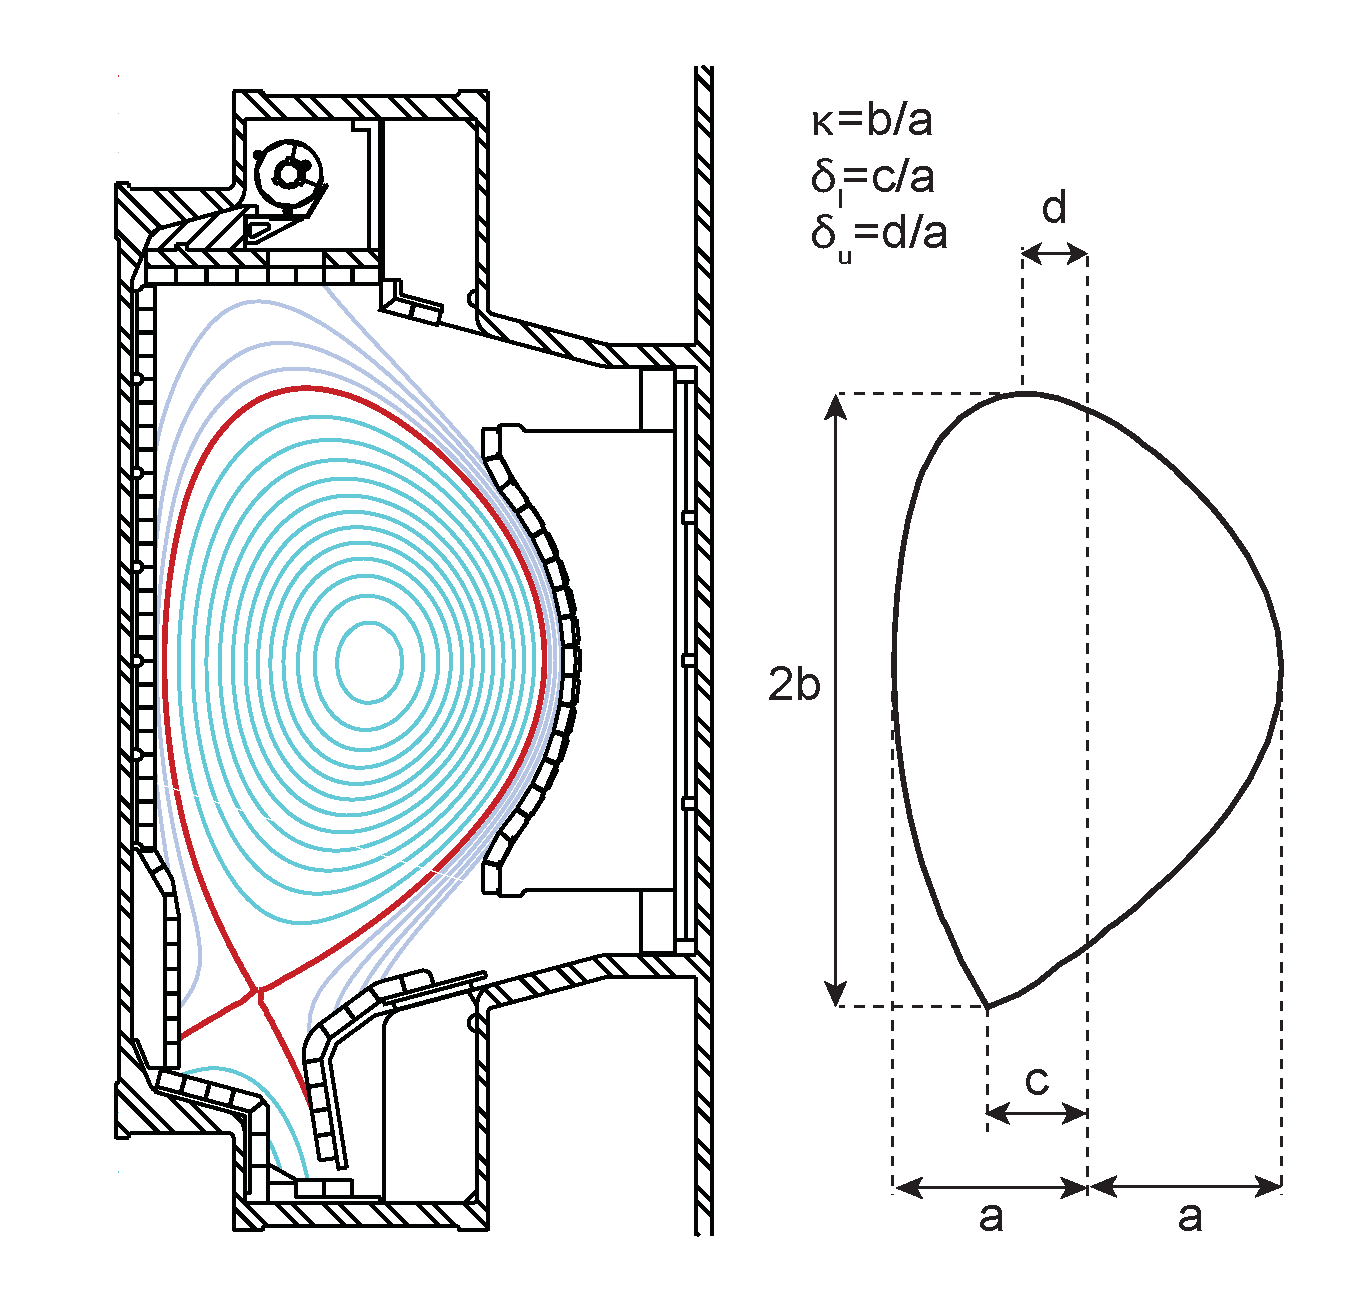
\includegraphics[width=150mm]{graphics/Introduction/shaping.pdf}}{\caption{Cross-section of a tokamak plasma, illustrating closed magnetic flux surfaces (light blue), the last closed flux surface (red), and surfaces with open magnetic field lines (dark blue).  Definitions for plasma shaping parameters elongation $\kappa$, and upper and lower triangularity $\delta_u$, $\delta_l$ are shown at right.}\label{fig:intro_shaping}}
\end{figure}



\nicesectionending

%%%%%%%%%%%%%%%%%%%%%%%%%%%%%%%%%%%%%%%%%%%%%%%%%%%%

\section{Alcator C-Mod}\label{sec:intro_cmod}

\begin{figure}[p]
 \pushtooutside
 \ffigbox[\FBwidth]{\caption{Cutaway view of the Alcator C-Mod tokamak, including cryostat and ancillary structures, illustrating the extensive support structures necessary for compact, high-field operation.}\label{fig:alcator}}{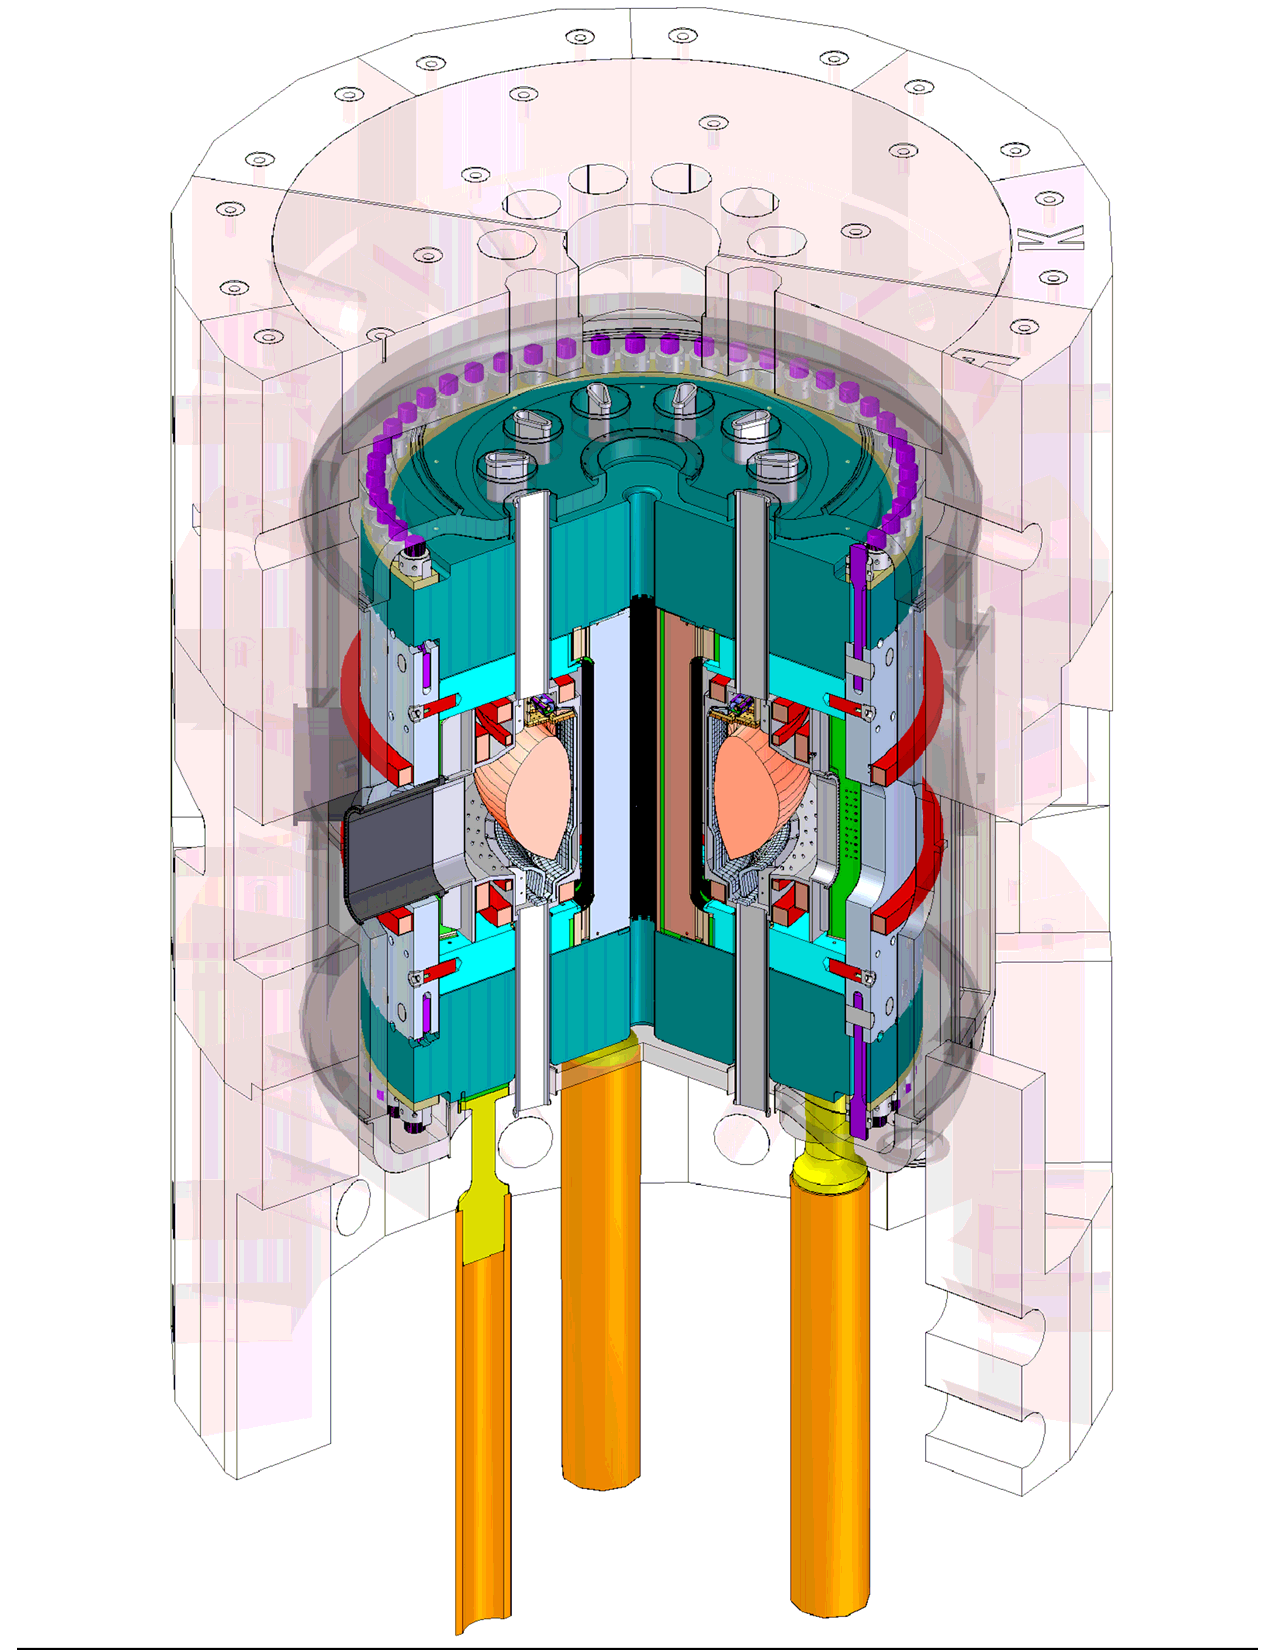
\includegraphics[width=165mm]{graphics/Introduction/alcator.pdf}}
\end{figure}

\begin{wraptable}{O}{0 pt}
 \ttabbox{\caption{Summary of Alcator C-Mod typical operating parameters.}\label{tab:cmod}}
  {\begin{tabular}{lc}
    \toprule
    \emph{parameter} & \emph{range}\\
    \midrule
    major radius & $\SI{0.67}{\meter}$ \\
    minor radius & $\SI{0.22}{\meter}$ \\
    toroidal field & $3 - \SI{8.1}{\tesla}$ \\
    plasma current & $\le \SI{2}{\mega\ampere}$ \\
    plasma density & $\le \SI{5e20}{m^{-3}}$ \\
    central temperature & $\le \SI{8}{\kilo\electronvolt}$ \\
    plasma pressure & $\le \SI{2}{\atmosphere}$ \\
    ICRF power & $\SI{6}{\mega\watt}$ \\
    LHRF power & $\SI{1}{\mega\watt}$ \\
    \bottomrule
   \end{tabular}}
\end{wraptable}

The data presented in this thesis were collected on the Alcator C-Mod tokamak \cite{Hutchinson1994,Greenwald2007} at the MIT Plasma Science and Fusion Center.  The Alcator series of tokamak experiments were designed as compact, high-field tokamaks.  Despite its small physical size ($\SI{67}{\centi\meter}$ major radius, $\SI{22}{\centi\meter}$ minor radius, considerably smaller than other major experiments), Alcator C-Mod plasmas are capable of reaching ITER- and reactor-relevant densities ($> \SI{1e20}{m^{-3}}$) and pressures ($>\SI{1}{\atmosphere}$).  This compact design is enabled by a very high toroidal magnetic field driven by liquid-Nitrogen-cooled copper coils, reaching as high as $\SI{8.1}{\tesla}$, with typical operation near $\SI{5.5}{\tesla}$, allowing reactor-relevant research in a small, cost-effective machine.  C-Mod plasmas are primarily heated by ion-cyclotron (ICRF) heating \cite{Takase1996}, with up to $\SI{6}{\mega\watt}$ of heating power, with an additional $\sim \SI{1}{\mega\watt}$ of 
lower-hybrid resonance (LHRF) power used for heating and DC current drive \cite{Wilson2009}.  A cutaway view of C-Mod, including support structures and the concrete ``igloo'' housing the cooling systems, is visible in \cref{fig:alcator}.  A detailed and annotated view of the C-Mod cross-section is shown in \cref{fig:alcator2}.

\begin{figure}[t]
 \pushtooutside
 \ffigbox[\FBwidth]{\caption{Cross-section of the C-Mod vacuum vessel, cryostat and diagnostic access ports, with toroidal-field and equilibrium-field magnetic coils labeled.  Also shown is the plasma position in a typical LSN shape, with strike points in the lower divertor shown..}\label{fig:alcator2}}{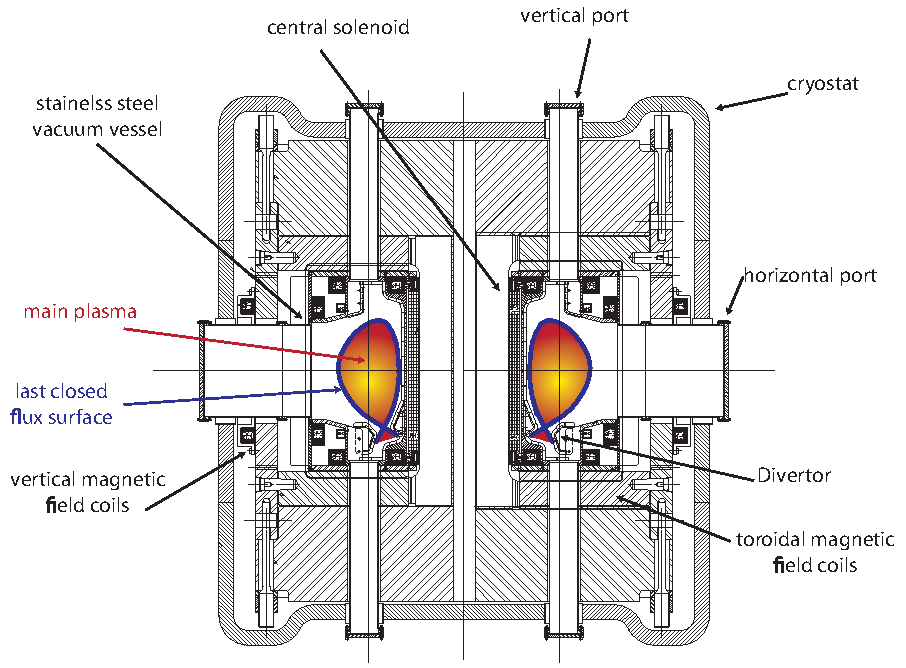
\includegraphics[width=150mm]{graphics/Introduction/cmod_xsec.pdf}}
\end{figure}

Due to their high plasma pressure and power density, C-Mod plasmas must exhaust a large heat flux, reaching levels comparable to that anticipated for ITER \cite{Loarte2007,Terry2007,LaBombard2011}.  To handle this heat flux, C-Mod operates entirely with high-$Z$ metal materials (primarily Molybdenum and Tungsten) for all plasma-facing surfaces.  In addition to its high heat tolerance and low erosion rates due to plasma contact, metal walls provide low retention of fuel gas at the edge -- metal walls are thus the leading candidate for ITER- and reactor-scale plasma-facing components.

The presence of a full high-$Z$ lower divertor and upper strike plate, as well as metal limiter walls, gives C-Mod great flexibility in attainable plasma shapes -- plasmas may be run in a lower-single null (LSN) shape with the plasma exhaust \gnote{elaborate on X-point nulls here, or in previous section?} striking the lower divertor (shown in \cref{fig:alcator2}, upper-single null (USN) exhausting into the upper strike plate, or in a limited shape where the scrape-off layer directly impinges on the plasma-facing wall.\nicesectionending

%%%%%%%%%%%%%%%%%%%%%%%%%%%%%%%%%%%%%%%%%%%%%%%%%%%%

\section{Confinement \& Transport}\label{sec:intro_confinement}

\subsection{Global Confinement}\label{subsec:intro_global}

The rate at which a fusion plasma bleeds off heat is described by a characteristic time scale, the energy confinement time $\tau_E$.  From basic power balance for the total plasma stored energy $W_p$,

\begin{equation}\label{eq:powerbalance}
 \frac{dW_p}{dt} = P_{in} - P_{out} = P_{in} - P_{rad} - \frac{W_p}{\tau_E}
\end{equation}

\noindent where $P_{in}$ is input heating power, from Ohmic heating $P_{Ohm} = I_p^2 R_{plasma}$, RF or beam auxiliary heating power $P_{aux}$, or self-heating of the plasma from fusion reactions.  In the case of the latter, note that as fusion neutrons are immediately lost into the blanket, only the energy carried by \emph{charged} fusion products contributes to fusion self-heating: in the case of $\si{D} - \si{T}$ fusion we denote this as the alpha heating power $P_{\alpha} = 1/5 \times P_{fusion}$ for the energy carried by the ${}^4\si{He}$ nucleus.  $P_{rad}$ denotes the power loss due to radiative (\eg Bremsstrahlung) effects, which are considered separately from the transport-driven heat losses encoded by $W_p/\tau_E$.  It is common to encapsulate these heat source and sink terms into a single net power,

\begin{equation}\label{eq:pnet}
 P_{net} = P_{Ohm} + P_{aux} + P_{fusion} - P_{rad} - \frac{dW_p}{dt}
\end{equation}

\noindent The radiative power loss is occasionally difficult to consistently determine experimentally, is in any case largely independent of operator control (as in the case of auxiliary heating power, or Ohmic power determined by the choice of plasma current) or bulk plasma performance (as in the suppression of turbulent heat losses in high-performance operation), and is relatively negligible at fusion conditions due to its weak scaling with temperature.  As such, it is alternately common to express the power as

\begin{equation}\label{eq:ploss}
 P_{loss} = P_{Ohm} + P_{aux} + P_{fusion} - \frac{dW_p}{dt} \Rightarrow P_{net} = P_{loss} - P_{rad}
\end{equation}

\noindent These definitions allow a simple relation for experimental energy confinement time,

\begin{equation}\label{eq:tauE}
 \tau_E = \frac{W_p}{P_{net}}
\end{equation}

\gnote{$\tau_{98}$ here, or in later section?}
\noindent In practice, the physics determining energy confinement are extremely complex; as such, working models for calculating $\tau_E$ from bulk parameters typically require an empirical power-law scaling.

A closer examination of the power balance equation, \cref{eq:powerbalance}, reveals an important figure of merit.  For a DT-burning fusion reactor, steady-state operation with plasma temperatures sustained by fusion self-heating (termed ``ignition'') is highly desirable.  At these conditions, Bremsstrahlung losses are small, so \cref{eq:powerbalance} reduces to simply

\begin{equation}\label{eq:powerbalance2}
 \frac{W_p}{\tau_E} = P_{\alpha}
\end{equation}

\noindent The alpha heating power is simply the fusion reaction rate $R_f = n_D n_T \langle \sigma v \rangle_{DT}$ times the energy carried by charged particles from a single reaction, $E_\alpha = 1/5 \times E_{fusion} = \SI{3.5}{\mega\electronvolt}$.  Quasineutrality (\cref{eq:quasineutral}) requires $n_e \approx n_D + n_T$.  As the reaction rate is optimized for a 50-50 fuel mix, the alpha heating power is thus given by

\begin{equation}\label{eq:palpha}
 P_{\alpha} = \frac{1}{4} n_e^2 \langle \sigma v \rangle E_\alpha
\end{equation}

\noindent The stored energy is defined by

\begin{equation}\label{eq:Wp}
 W_p = \frac{3}{2}p_{thermal}
\end{equation}

\noindent with the thermal pressure in the plasma given by

\begin{equation}\label{eq:pthermal}
 P_{thermal} = n_e T_e + n_D T_D + n_T T_T = 2 n_e T_e
\end{equation}

\noindent assuming the condition above on the electron and ion densities, and assuming temperature equilibration $T_e \approx T_D \approx T_T$.  This, then, implies $W_p = 3 n_e T_e$ (a convenient expression, as electron quantities are typically more readily measured in plasma experiments).  Power balance at ignition then requires

\begin{equation}\label{powerbalance3}
 \frac{3n_e T_e}{\tau_E} = \frac{1}{4} n_e^2 \langle \sigma v \rangle E_\alpha
\end{equation}

\noindent thus simplifying to the Lawson Criterion \note{cite this!}\gnote{citation for Lawson criterion}

\begin{equation}\label{eq:lawson}
 n_e \tau_E = \frac{12 T_e}{\langle \sigma v \rangle E_\alpha}
\end{equation}

\noindent Scaling both sides by $2T_e$ gives the ``triple product,''

\begin{equation}\label{eq:tripleproduct}
 2 n_e T_e \tau_E = p \tau_E = \frac{24 T_e^2}{\langle \sigma v \rangle E_\alpha}
\end{equation}

\noindent an important figure of merit for a reactor that is optimized at $T_e \approx \SI{15}{\kilo\electronvolt}$ with a value of $p \tau_E \approx \SI{8.3}{\atmosphere\cdot\second}$, setting target parameters for a fusion reactor.

\gnote{cite Freidberg for beta limit?}
However, the maximum attainable thermal pressure in a tokamak is limited by a global MHD stability limit expressed in terms of the normalized pressure

\begin{equation}\label{eq:beta}
 \beta = \frac{2 \mu_0 p}{B^2}
\end{equation}

\noindent which encodes the ratio of thermal pressure to magnetic pressure $B^2/2\mu_0$ (equivalently, the ratio of thermal and magnetic stored energy) -- a normalization that also falls naturally out of solutions to the MHD equilibrium, \cref{eq:MHDeq}.  Although the maximum stable pressure may be increased with higher plasma current and toroidal field (motivating high-field design for tokamaks), reactor-scale operation requires increased energy confinement (\ie higher values for $\tau_E$) to reach the triple-product target.

\subsection{Transport Barriers}\label{subsec:intro_barriers}

\gnote{mention $\tau_E$ earlier, give a sense of how to globally improve confinement?}Global improvement to energy confinement may be achieved through local modification of the transport of energy or particles out of the plasma, achieved via structures termed \emph{transport barriers}.  While the physics driving the formation of transport barriers is not entirely understood\note{how deep to go with this?}, the effect is evidently caused by sheared flows in the plasma -- these break up the turbulent ``eddies'' driving much of the energy or particle transport through the plasma, locally reducing transport drive in the sheared region.  

The effect on the transport is clearly evident from a diffusive transport model, given by

\begin{equation}\label{eq:diffusion}
 \frac{\partial Q}{\partial t} = \nabla \cdot \left( D_Q \nabla Q \right) + R_Q
\end{equation}

\noindent for a general parameter $Q(\vec{x},t)$ with accompanying diffusion coefficient $D_Q$ and net source/sink term $R_Q$.  We may consider a one-dimensional ``toy model'' of diffusion with a simple constant source term, given in steady state by

\begin{equation}\label{eq:diffusion2}
 \frac{d}{dx} \left( D_Q \frac{dQ}{dx} \right) + R_Q = 0
\end{equation}

\noindent The solution to this model for two sample diffusion coefficients is given in \cref{fig:intro_transport}.  A simple constant diffusion coefficient $D_Q$ produces a profile with weak slope, whereas an order-of-magnitude drop in $D_Q$ near the edge (consistent with experimentally-observed values of diffusion coefficients in transport barriers) produces a region with a steep gradient in $Q$

% \begin{wrapfigure}{O}[\marginparwidth+\marginparsep]{70mm}
%  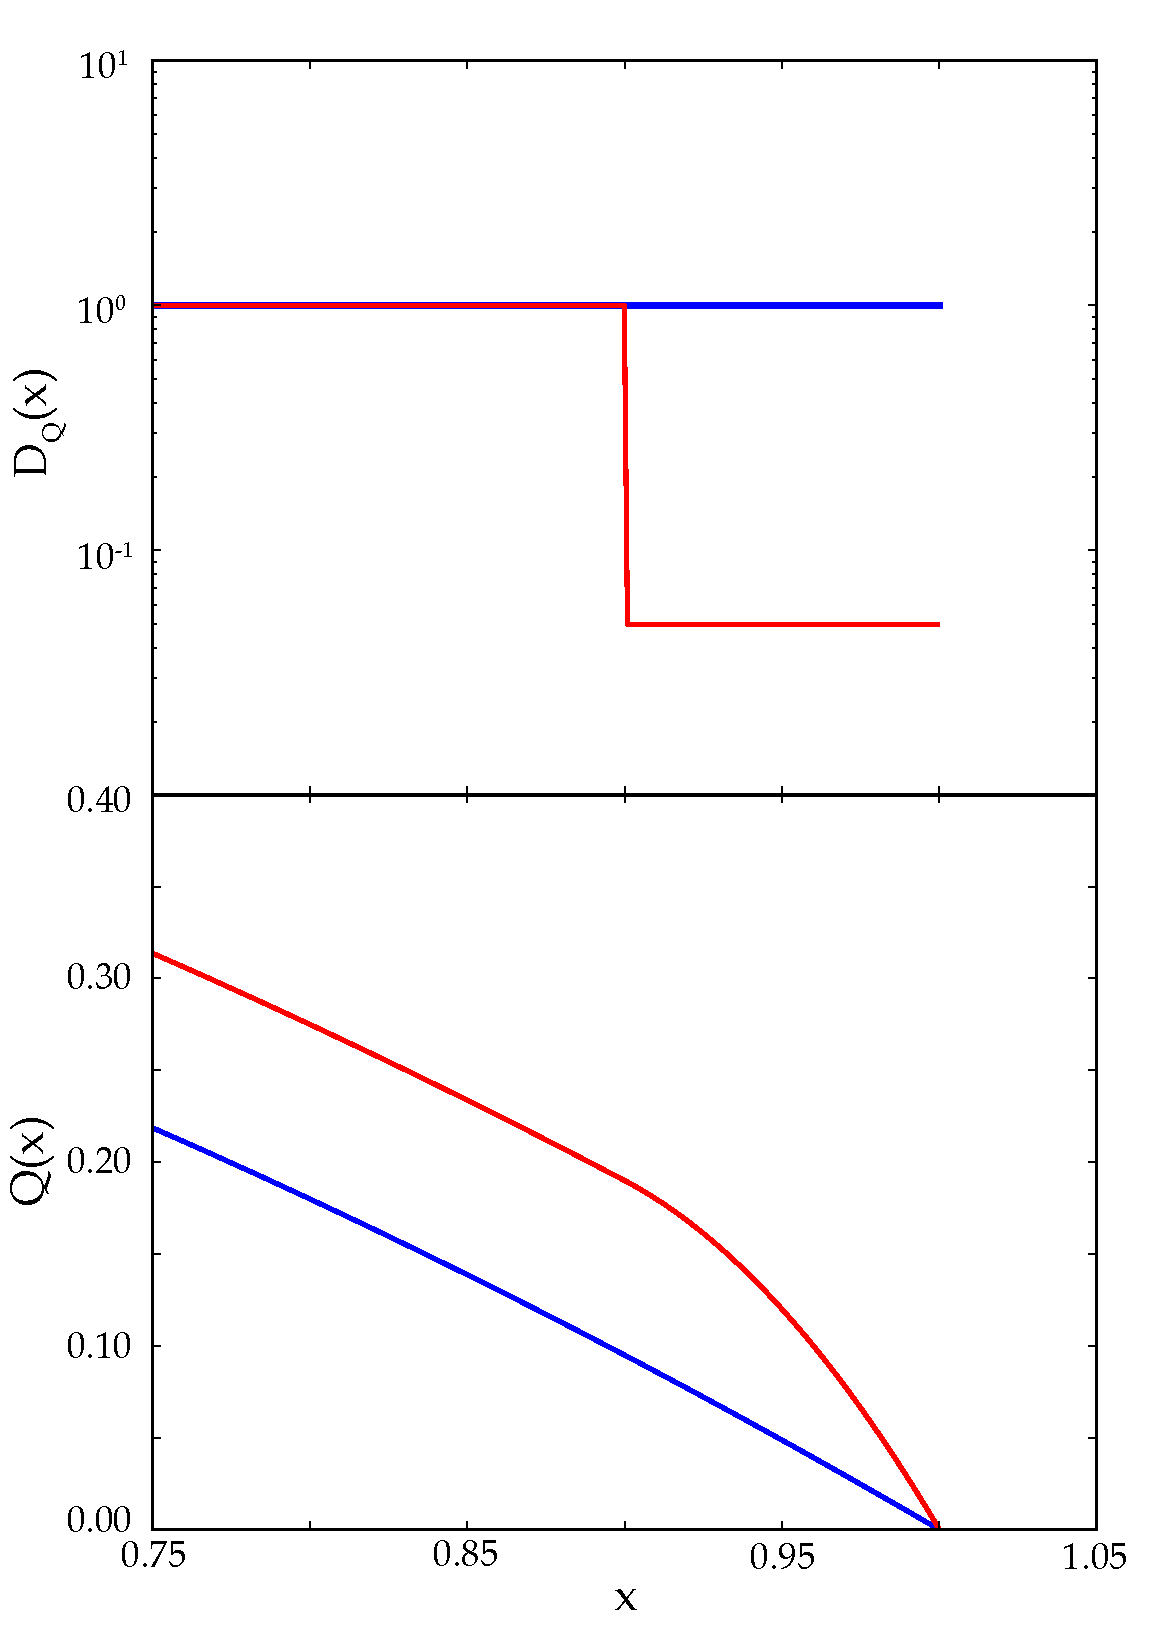
\includegraphics[width=70mm]{graphics/Introduction/transport.pdf}
%  \caption{Diffusion coefficients and plasma profiles for a ``toy model'' 1D diffusion equation with a general parameter $Q(x)$ and accompanying diffusion coefficient $D_Q(x)$.  An order-of-magnitude drop in $D_Q$ (of consistent magnitude with experimentally observed edge transport barrier behavior) produces a steep-gradient region in the edge compared to a constant $D_Q$.}
%  \label{fig:intro_transport}
% \end{wrapfigure}

%check this for caption on other side?
\begin{figure}[h]
 \pushtooutside
 \fcapside[50mm]{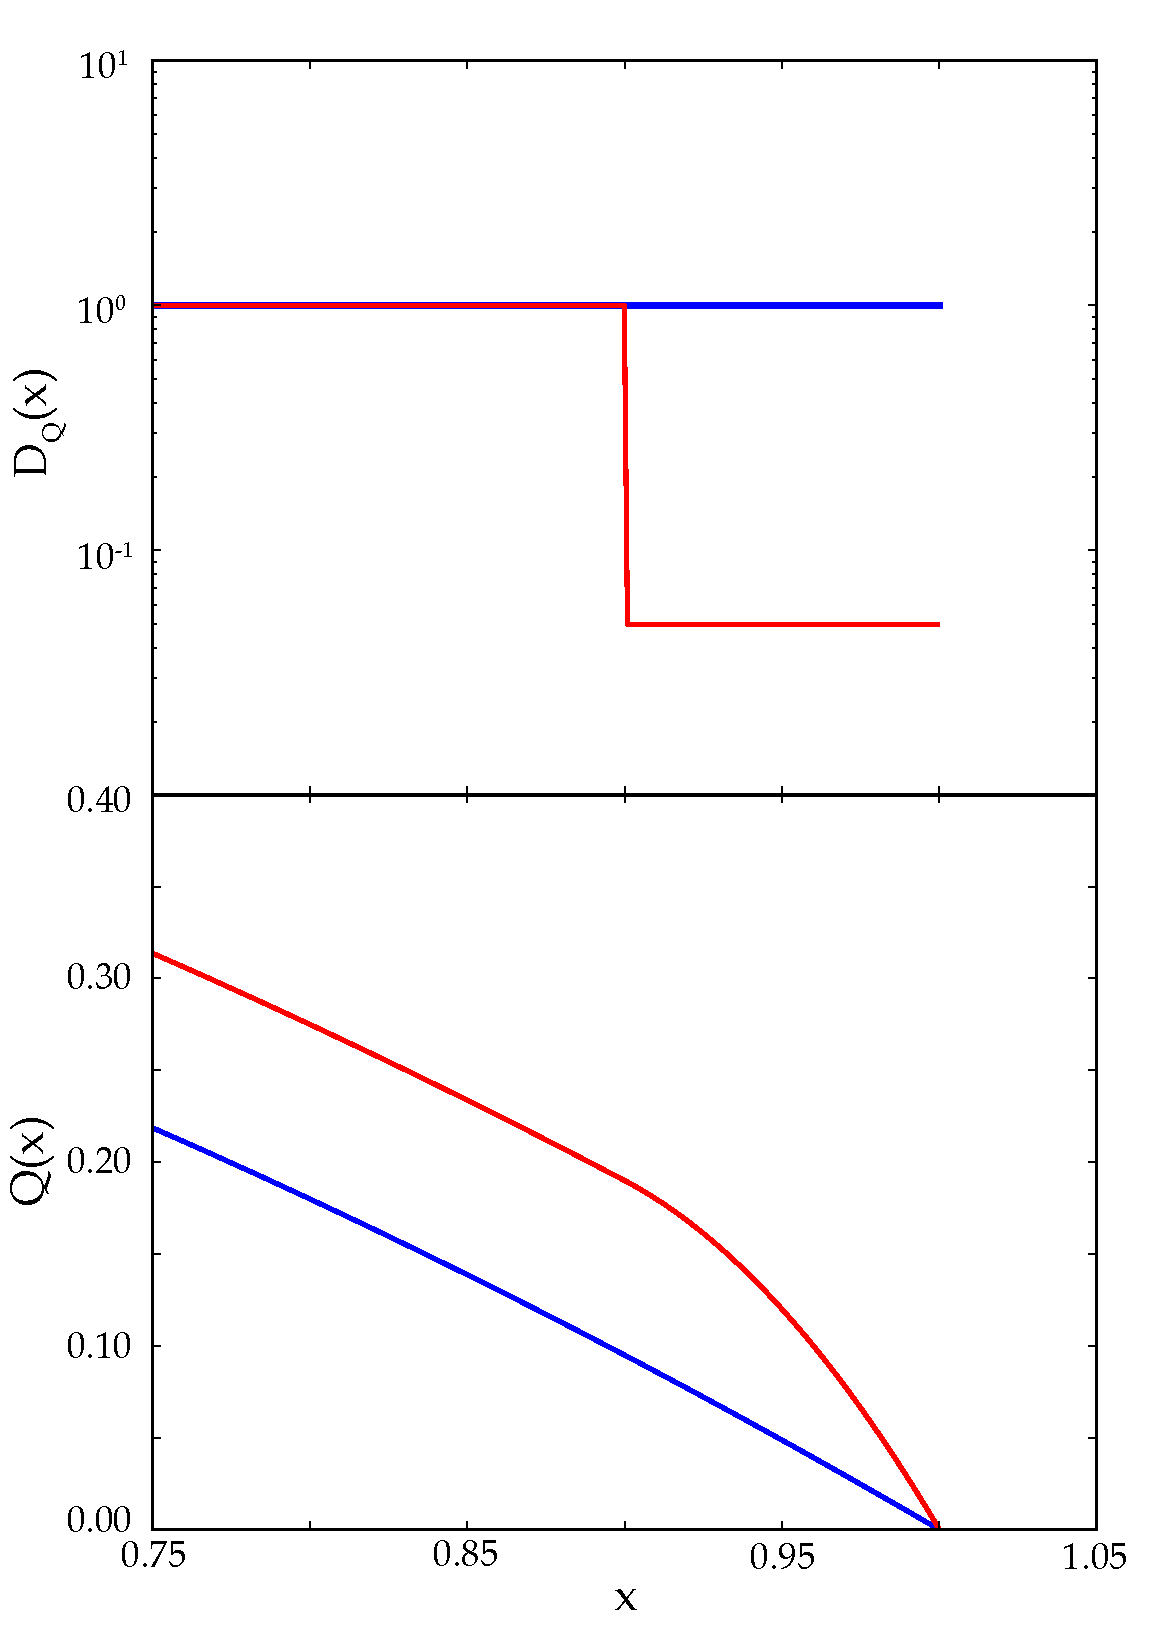
\includegraphics[width=85mm]{graphics/Introduction/transport.pdf}}{\caption{Diffusion coefficients and plasma profiles for a ``toy model'' 1D diffusion equation, \cref{eq:diffusion2}, with a general parameter $Q(x)$ and accompanying diffusion coefficient $D_Q(x)$.  An order-of-magnitude drop in $D_Q$ (of consistent magnitude with experimentally observed edge transport barrier behavior), shown in red, produces a steep-gradient region in the edge compared to a constant $D_Q$, shown in blue.}\label{fig:intro_transport}}
\end{figure}



\nicesectionending

%%%%%%%%%%%%%%%%%%%%%%%%%%%%%%%%%%%%%%%%%%%%%%%%%%%%

\section{Goals \& Outline}\label{sec:intro_outline}



\nicechapterending

%%%%%%%%%%%%%%%%%%%%%%%%%%%%%%%%%%%%%%%%%%%%%%%%%%%%

% do per-chapter bibliographies, or one big one?
\bibliographystyle{../plainurl}
\bibliography{../references} 